\label{Chapter:Intro:Rep:Learning}

\emph{Machine learning} is the field of computer science that studies algorithms that improve automatically through experience from examples. 
These algorithms allow computers to discover how to
perform tasks without being explicitly programmed to do so. For the computers to learn, it is mandatory that a finite set of data (or dataset) $\D$ is available. 

This data can be \emph{labeled} or \emph{unlabeled}. Labeled comes in pairs $(x_i,y_i)$, where $x_i$ is a datapoint and $y_i \in Y$ is a specific label that has previously been assigned to $x_i$. Usually, $Y$ is a set of classes or real values.
Unlabeled data is the kind of data that does not have a label or class associated to it, so it is just $x_i \in \R^d$. 

Depending on how the available data the machine learning approaches can be divided into two broad categories:
\begin{enumerate}
    \item \emph{Supervised learning}. In this category the goal is to use the labeled data in order to find a function that maps the dataset to the set of classes or real values. That is a function $g:\D \to Y$. 
    An example of supervised learning is image classification: giving a label to an image.
    \item \emph{Unsupervised learning}. In ths case, the data is unlabeled, so the approach is completely different. Usually, the goal here is to discover hidden patterns in data or to learn features from it.
    An example of this kind of learning is K means, which consists of clustering the data in $k$ groups. It is also known as \emph{self-supervised} learning.

\end{enumerate}

When machine learning was born (around the 1950s), all the problems were related to supervised learning. Then, in the 1970s, \emph{backpropagation} was developed allowing models to adapt to new situations much faster. Since then, diverse algorithms that manage to find truly complex $f$ functions have been developed and new problems have emerged. Supervised learning has a huge cost (economic, time): all the examples in the dataset must be labeled. This is so expensive due to the fact that labeling examples is a slow process, and has to be done mostly manually. 

Also, a worrying generalization problem was discovered in a very simple classification problem: discriminating between cows and camels images in different environments \citep{beery2018recognition}. The original data had a lack of different environments, that is, all the caws had grass in the background and all camels had a desert in the background. The models obtained really good results in images where the context (in this case, the background) was the same as the one we trained with. However, when we changed the context, eg: placed a cow in the snow instead of in the grass, the performance of the models drastically decreased. This led to the discovery that the models were simply using the context to discriminate from the different animals rather than focusing on the important part of the image, the animal.

\emph{Unsupervised learning} avoids these problems by trying to infer properties (or features) of the data using the \emph{unlabeled} dataset. By not needing to have the labels of the examples, companies can save money and time that they would have invested creating a label for each individual example. Also, by discovering general features about the context the models, the general context of the data is less important than it sometimes happens to be in supervised learning.

When the dimension of the data is high, for instance when treating images computationally, it is usual to first create a \emph{representation} of the input data. A representation is a lower dimensional vector that aims to contain the same features that the original data contained. More formally, if $x$ is a datapoint in a dataset $\D \subset \R^d$, a \emph{representation} of $x$ is a vector $r \in \R^n$ (usually, $n \leq d$), that shares information with the datapoint $x$. 


\emph{Features} are parts or patterns of an datapoint $x \in \D$ that help to identify it. In fact, it is desirable that this attribute is shared by all independent units that represent the same object. For instance, if we consider an image of any square, we should be able to identify 4 corners and 4 edges. These could be features of a square.

Representation learning is a set of techniques that allow a system to produce representations that help in the later tasks such as feature detection or classification.
The performance of machine learning methods is heavily dependent on the choice of data features \citep{bengio_representation_2014}. This is why most of the current 
effort in machine learning focuses on designing preprocessing and data transformation that lead to good quality representations. A representation will be of good quality when its features
produce good results when we evaluate the \emph{accuracy} of our model.

The main goal in representation learning is to obtain features of the data that are generally good for either of the supervised tasks. These tasks are usually called \emph{downstream tasks}. That is, we would like to obtain
a representation that is either good for image classification (giving an image a label of what we can see in it) or image captioning (producing a text that describes the image).

The features of the data that are invariant through time are very useful for machine learning models. In \citep{wiskott_slow_2002}, \emph{slow features} are presented. Slow features are defined as features of a signal 
(which can be the input of a model) that vary slowly during time. That means, if $\bm{X}$ is a \emph{time series}\footnotemark, we will try to find any number of features in $\bm{X}$ that vary the most slowly.
These kind of features are the most interesting ones when creating representations, since they give an abstract view of the original data.


%------------- Footnotemark
\footnotetext{A time series is an ordered sequence of values of a random variable at, usually, equally spaced time intervals.}
%----------------------

\begin{nexample} In computer vision, the value of the pixels in an image can vary fast. For instance, if we have a zebra on a video and the zebra is moving from one side of the image to the other, due 
to the black stripes of this animal, the pixels will fast change from black to white and vice versa, so value of pixels is probably not a good feature to choose as an slow feature. However, there will always
be a zebra on the image, so the feature that indicates that there is a zebra on the image will stay positive throughout all the video, so we can say that this is a slow feature.
\end{nexample}

We will be studying different models that try to learn representations from raw data without labels, as we have mentioned. We usually need a function that measures what is the penalty that the model gets for a choice of a parameter.
This is called a \emph{loss function}, that we will want to optimize. 


%% ORIGINAL INTRO
% --------------------------

In the search for a suitable loss function, a first approach to the problem was to use concepts from information theory. Ideally, we would like the original data and the representation created to contain the same information. A way of measuring this is using the \emph{mutual information} $I(X,Z)$ between the input $X$ and the representation $Z$. The mutual information is expressed as:
\[
I(X,Z) = H(X) - H(X|Z),
\]
where $H(X)$ is the entropy of $X$ and $H(X|Z)$ is the conditional entropy.

\begin{figure}[H]
    \centering
    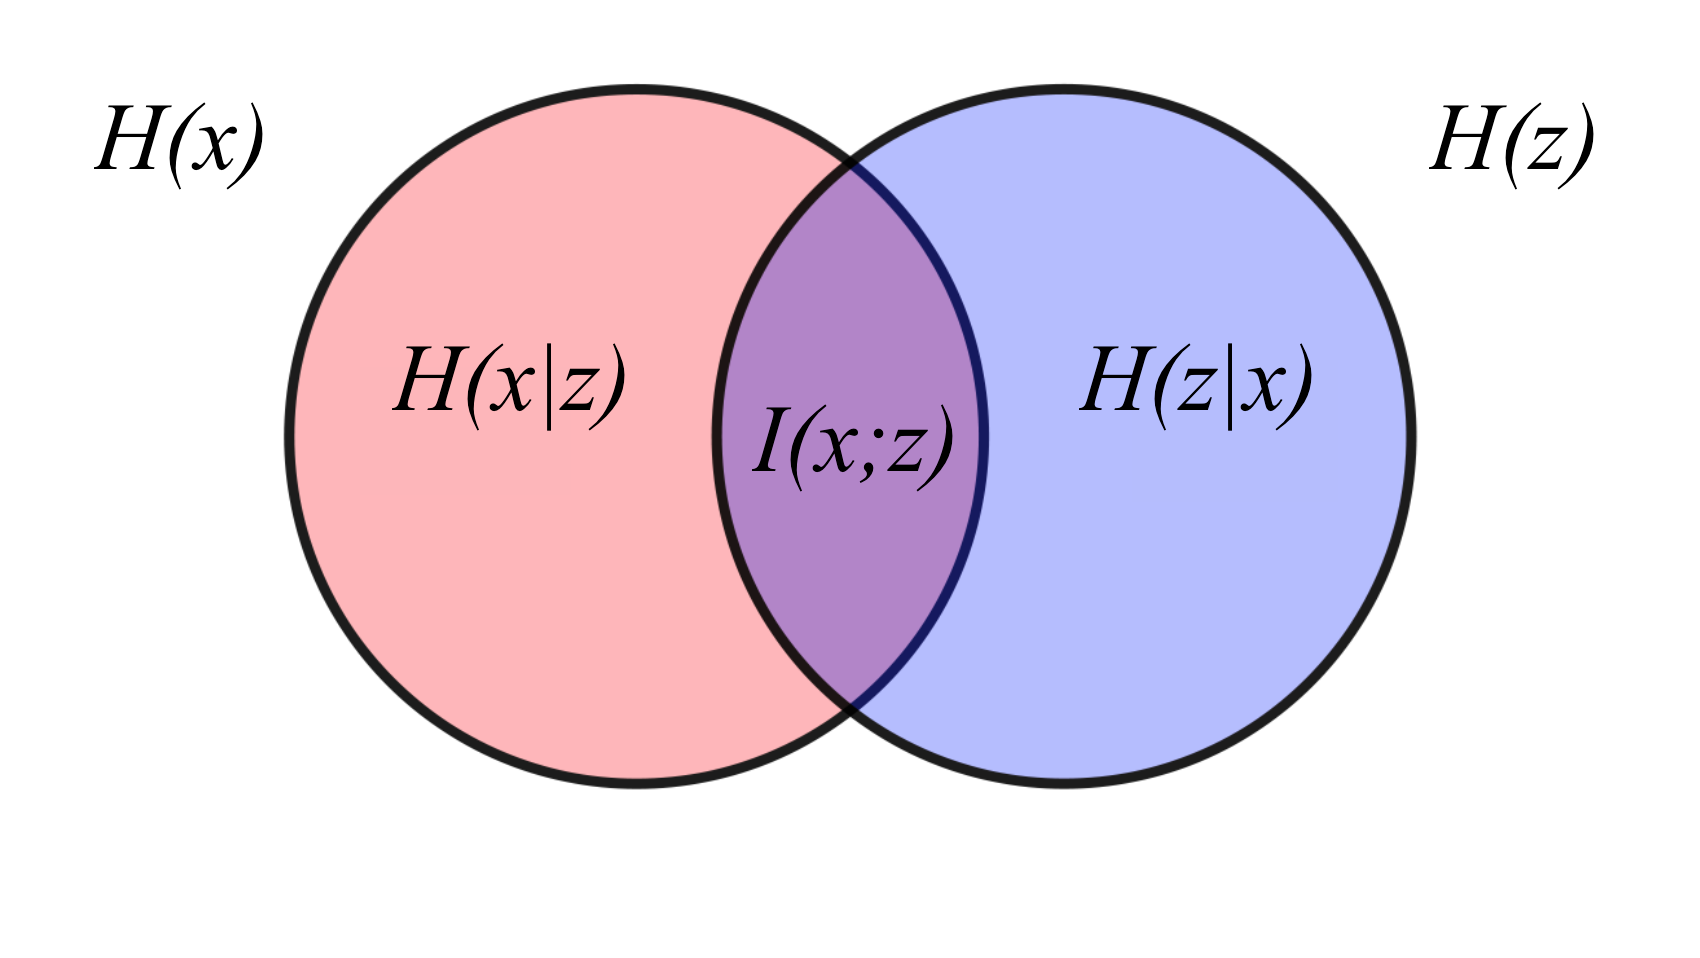
\includegraphics[scale=0.25]{mutual-info}
    \caption{Venn Diagram showing the relationships between the entropies and the conditional entropies of random variables $X$ and $Z$.}
\end{figure}

Since the entropy is a way of measuring ``\emph{how surprising is that an event occurs}'' (this is explained in this document), intuitively the mutual information measures the decrease of uncertainty that we obtain in $X$ when we know that $Z$ has occurred.

Calculating the mutual information between two variables, however, is not an computationally easy problem. Because of this, a way to approach the mutual information maximization is by obtaining lower bounds and maximizing them. Although a few more bounds are proved in this document, we remark the \emph{Contrastive Lower Bound} on the mutual information, which is expressed as follows:
\[
I(X,Z)  \geq - \ell(\theta) + \log N,
\]
where $\ell(\theta)$ refers to the contrastive loss. In short, the \emph{contrastive learning} problem consists of, given elements obtained from one distribution $P$ (considered as positive samples) and elements obtained from a different distribution $Q$ (considered as negative samples), learning how to discriminate between the elements of the different distributions. In order to do this, the recently mentioned contrastive loss is used, which usually takes the form
\[
\ell_{i,j} = -  \log \frac{f(x_i,x_j)}{\sum_{x_k \in X}f(x_i,x_k)},
\] 
where $(x_i,x_j)$ is a positive pair. Intuitively, contrastive loss takes the output of the network for a positive example and calculates its distance (using the function $f$) to an example of the same class and contrasts that with the distance to negative examples. In other words, the loss is low if positive examples are encoded to similar representations and negative examples are encoded to different representations. The use of this contrastive loss maximizing the mutual information had a huge impact on the state of art results of representation learning in 2018 \citep{oord_representation_2019}, achieving very promising results.

However, during the development of this work (around July 2020), this drastically changed. New papers  \citep{chen_simple_2020, grill2020bootstrap} appeared stating that the success of the methods that were maximizing mutual information between the input and its representation was not caused by mutual information, but by the specific form that the contrastive loss has.

With this papers, new frameworks for representation learning appeared. These frameworks provided an ingenious way to apply  the contrastive learning set up to representation learning. This technique consists of presenting different perspectives of the same image to two different encoders (the neural networks that learns how to transform the input to a representation) different \emph{perspectives} (or, being technical, \emph{data augmentations}) of the same image and, later, trying to minimize some sort of distance between these views.  

To achieve this, these perspectives are obtained by applying transformations to the original image. It is shown that the chosen transformations and how to sequence them before passing the transformed image to the neural network really affects the performance of the models.

All this considered, the interest of this work  speaks on its own. Being able to train networks that learn representations that are good enough on its own to perform downstream tasks without needing the supervision of having the labels of the data opens a world of possibilities in many areas. For instance, many insurance companies need to pay their workers to label large amounts of  different insurance bills that they offer to their clients. With the advances presented in this work, these companies would only have to label a very small amount of images to be able to classify the representations obtained by the frameworks.


\section*{Main goals and results achieved}

The main goals of this bachelor's thesis were:
\begin{enumerate}
\item To study, understand and present the basic concepts and properties of \emph{mutual information}, which is in the field of \emph{Information Theory.} Also, related to this, to present some lower bounds that can be used to maximize the mutual information between two random variables.
\item To study the \emph{noise contrastive estimation} problem, and how it is applied to machine learning.

\item To test the most important frameworks that achieve the current state of art results in representation learning. 
\end{enumerate}

The first two goals were successful. For the latter goal, two different frameworks were tested: \lstinline{SimCLR} and \lstinline{BYOL}. 

Different executions were made for each one, trying to find the set of parameters for being able to obtain a high classification accuracy on a specific dataset. The selection of the chosen hyperparameters was argued and the limitations and problems we face are also presented. This way, I gained not only a deep understanding of the representation learning problem and how it is solved, but also in computational capability of the used hardware, so that a plausible future plan could be to improve the results obtained by making use of even better computational resources.
